\section{Análisis del problema}

\subsection{Elección de la temática: el juego de la oca}

Antes de pasar a la etapa de diseño y desarrollo, se debe elegir el tipo de juego a implementar, teniendo en cuenta factores de viabilidad tanto del ámbito tecnológico como del psicológico (¿es apropiado para el grupo demográfico al que va dirigido?).

Como se ha visto en la sección \textit{2.1.3.}, los juegos tradiciones pueden servir como fuente de inspiración para lo que se busca en este proyecto. Sin embargo, existe una gran cantidad de juegos de mesa populares entre los adultos mayores, como es el caso del parchís, el scrabble, el memorama, el dominó, etc. Entonces, ¿por qué decantarse por el juego de la oca?

El principal motivo es la flexibilidad que permite a la hora de diseñar un juego que cumpla unos objetivos específicos. Un ejemplo de ello es la iniciativa de un Centro de Educación Primaria en Murcia, que implementó un programa innovador para la evaluación de las habilidades motrices del estudiantado. \parencite{experienciaOca}

El proceso fue el siguiente: se diseñaron tres tableros de la oca, que se correspondían con los tres ciclos escolares que participaron en el experimento. Cada uno, además de las casillas especiales del juego original (oca, puente, calavera...), disponía de una serie de actividades físicas para poner a prueba a los participantes, entre las que se encuentran: el lanzamiento y captura de objetos, ejercicios de malabares y equilibrio y cooperación con los compañeros.

\begin{figure}[h]
	\centering
	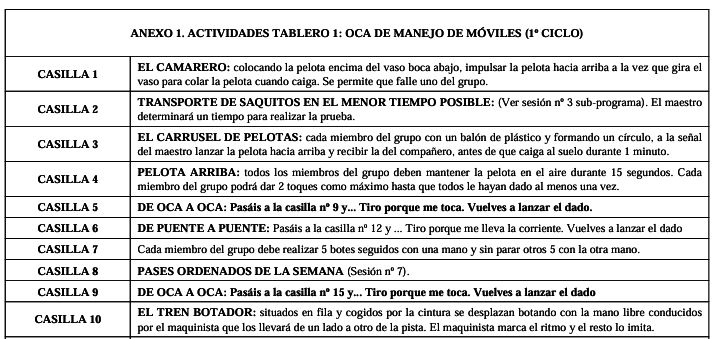
\includegraphics[width=1\textwidth]{imgs/casillas-oca-primaria.JPG}
	\caption{Diseño de la oca para evaluar las habilidades motoras en Educación Primaria \parencite{experienciaOca}}
	\label{fig:casillas-oca-primaria}
\end{figure}

\begin{figure}[h]
	\centering
	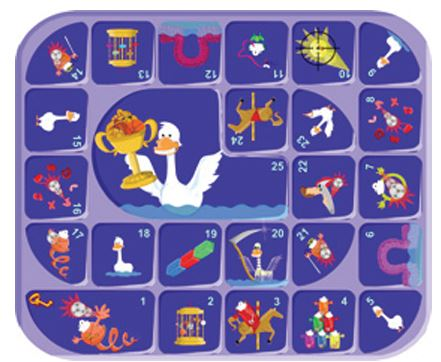
\includegraphics[width=0.45\textwidth]{imgs/oca-primaria.JPG}
	\caption{Tablero completo correspondiente a las casillas de la figura superior \parencite{experienciaOca}}
	\label{fig:oca-primaria}
\end{figure}


Esta medida tuvo gran éxito, pues los seguimientos del progreso de los participantes mostraron una mejoría general en sus destrezas físicas y capacidad de trabajo en equipo, así como una participación activa por parte de los estudiantes de Primaria que no se había registrado hasta el momento.

Por tanto, se ha querido replicar de alguna manera ese enfoque, trasladándolo a un contexto donde el grupo objetivo son los adultos mayores, y teniendo en cuenta la diversidad que puede existir dentro del mismo. 

Partiendo de la estructura del tablero original, hay una mayor probabilidad de que los adultos mayores estén familiarizados con su diseño y las reglas básicas, lo que puede contribuir a una experiencia de juego positiva y fluida.

\begin{figure}[H]
	\centering
	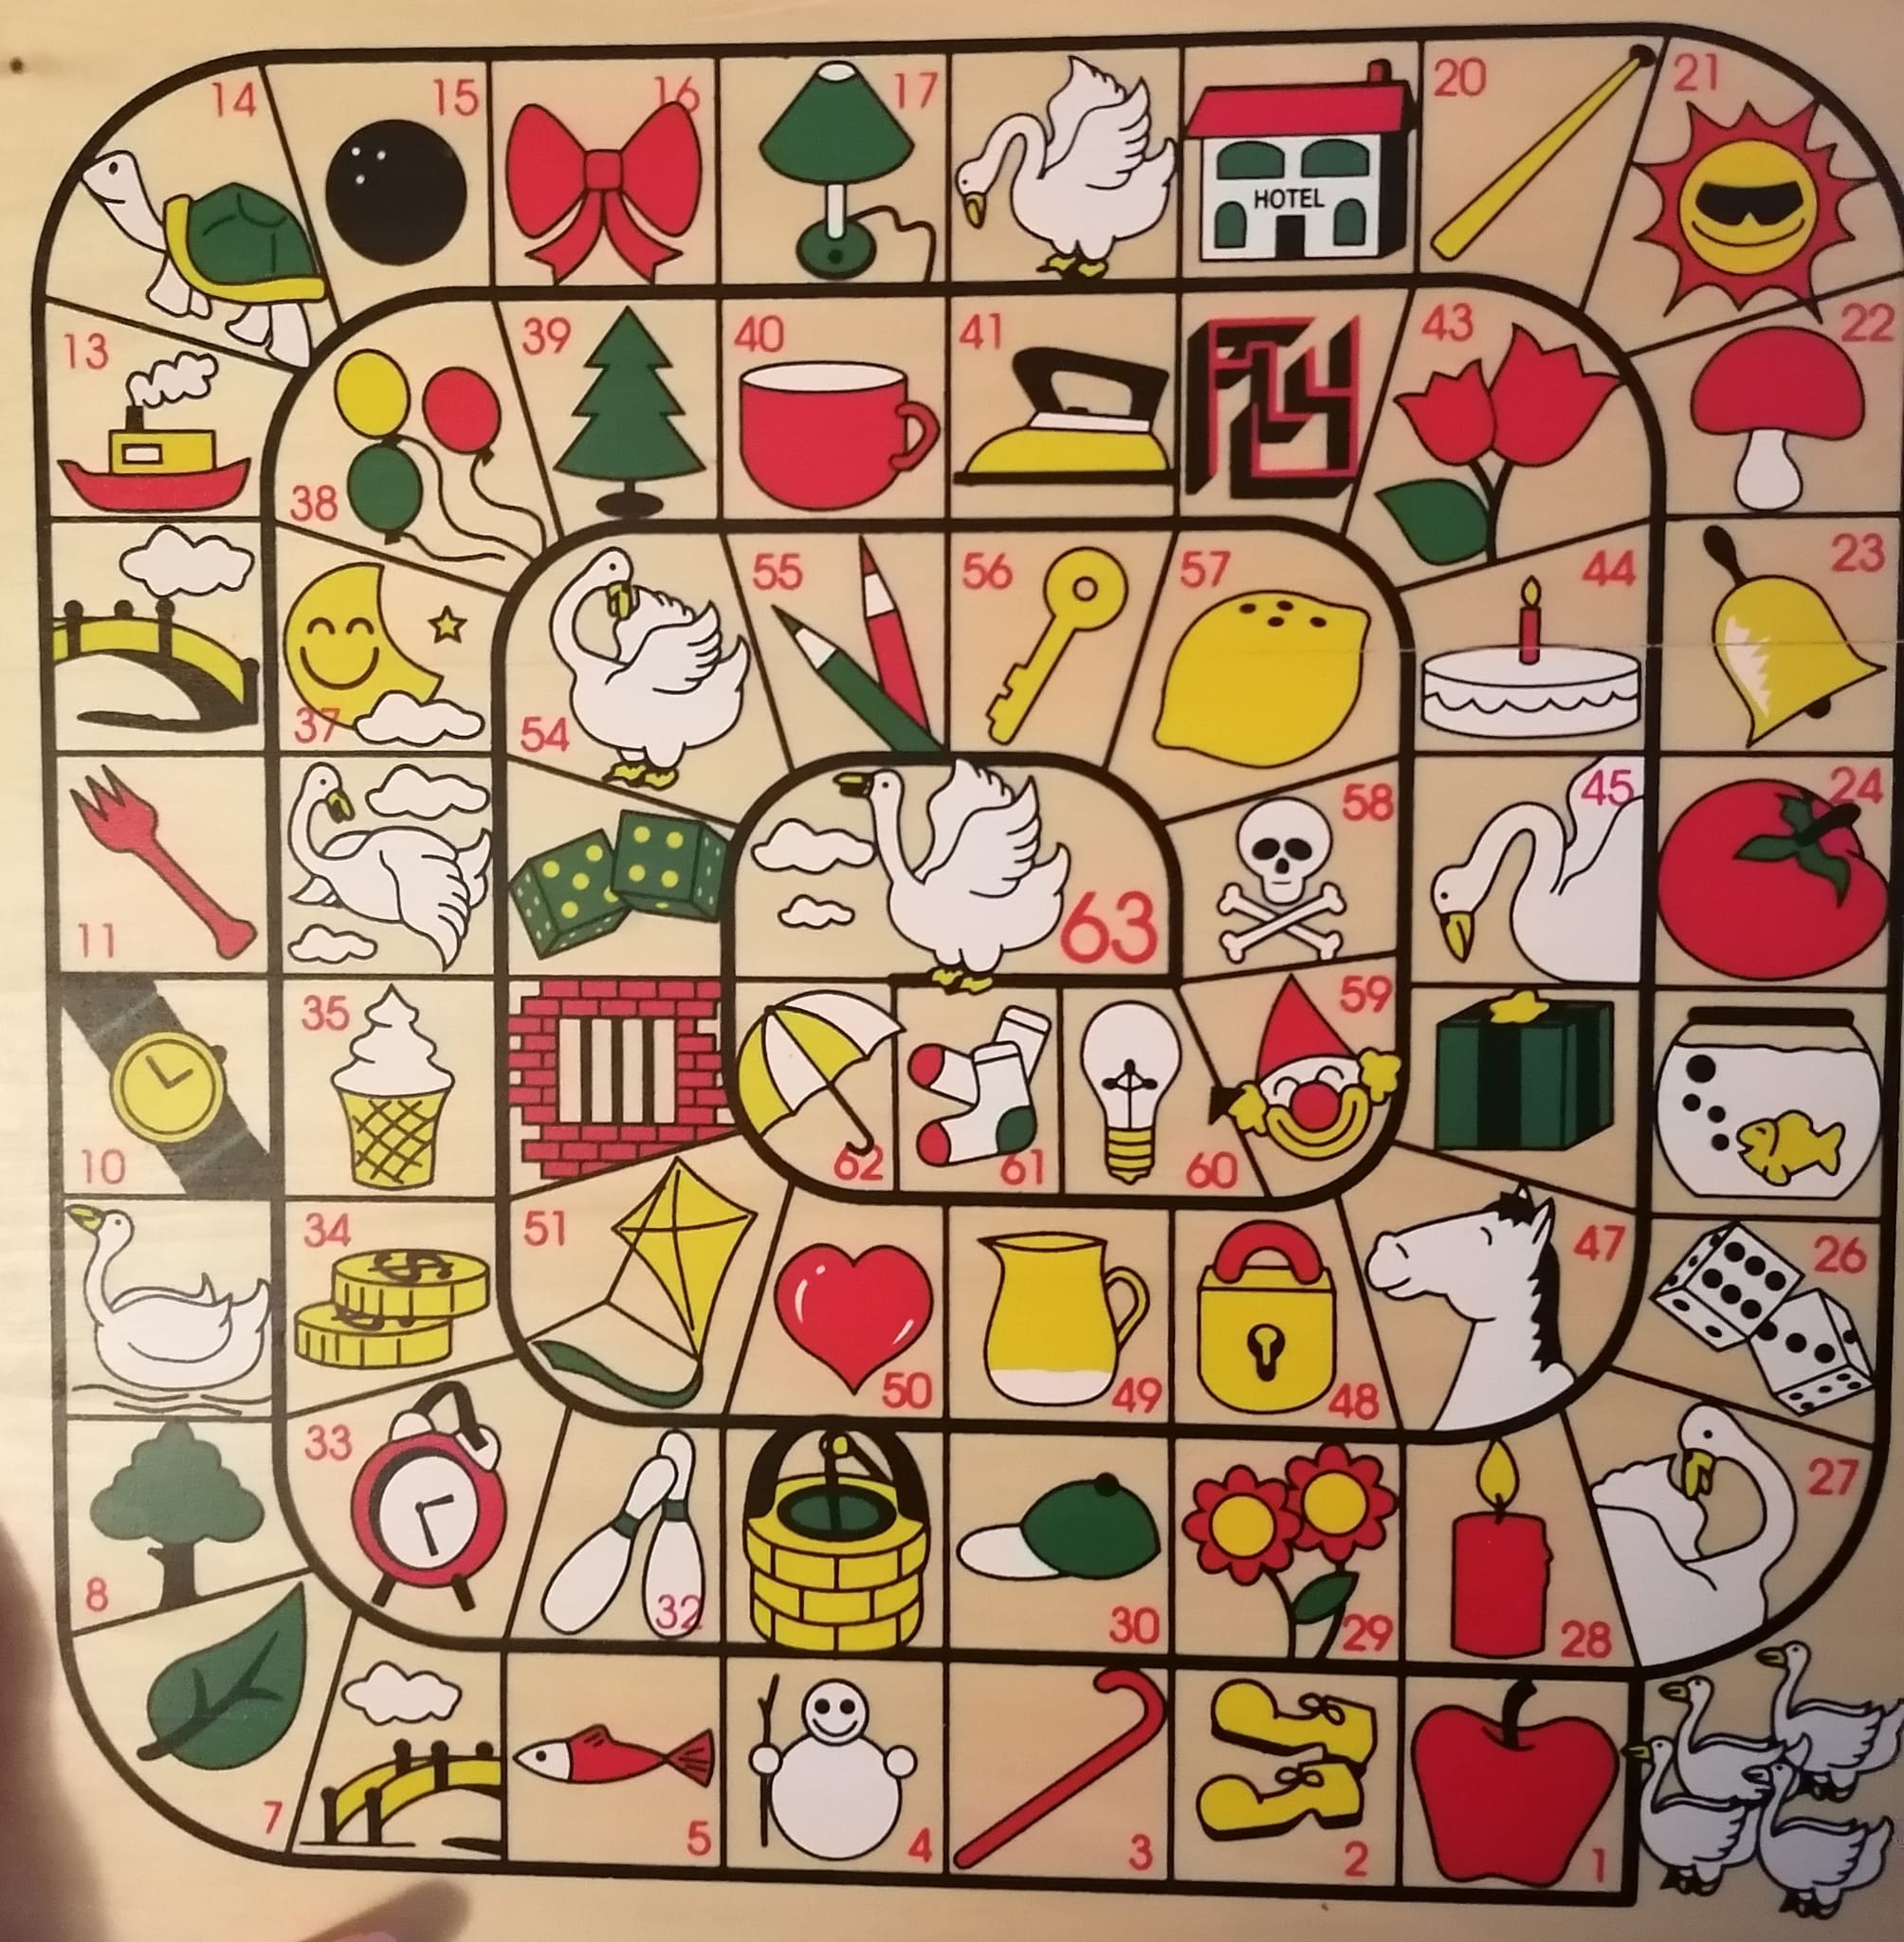
\includegraphics[width=0.7\textwidth]{imgs/oca-tradicional.jpg}
	\caption{Un tablero del juego tradicional de la oca}
	\label{fig:oca-tradicional}
\end{figure}


Sin embargo, al igual que la oca adaptada para estudiantes de Educación Primaria vista anteriormente, no se tratará de una oca tradicional cualquiera. 

Pues aparte de las casillas originales y el objetivo de llegar a la meta, incluirá un sistema de puntos, añadiendo un subobjetivo: el de conseguir la mayor puntuación antes de que termine la partida. Los participantes del juego podrán incrementar su marcador a través de una serie de minijuegos, que serán desencadenados cuando los jugadores caigan en determinadas casillas especiales.

También debe evaluarse la viabilidad de los minijuegos propuestos dentro del juego principal, que es la oca, para lo que se ha consultado con un equipo de psicólogos que han participado en varias experiencias de residencias.

\subsubsection{Lista de minijuegos dentro de la oca}
Dada la dificultad de implementar algunos en base a las limitaciones de los dispositivos Alexa, y para evitar saturar a los participantes con demasiadas mecánicas nuevas, se han elegido los siguientes cinco minijuegos:

\begin{enumerate}
	\item \textbf{Preguntas de Trivial V/F}: pondrán a prueba los conocimientos generales de los participantes. Se abordarán categorías distintas (geografía, historia, ciencia, arte y cultura…) pero siempre habrá dos opciones de respuesta, \textit{verdadero} o \textit{falso}. Si se acierta, se obtienen puntos, y si no, Alexa proporcionará una breve explicación de la respuesta correcta.
	\begin{itemize}
		\item Alexa: \textit{¿Oceanía es el continente más pequeño de todos?}
		\item Agustín: \textit{Verdadero.}
		\item Alexa: \textit{¡Correcto! Has ganado 10 puntos.}
		
		Alternativamente...
		\item Agustín: \textit{Falso.}
		\item Alexa: \textit{Incorrecto, el continente más pequeño del mundo es Oceanía, con 9.000.000 km² de superficie.}
	\end{itemize}
	
	\item \textbf{Conoce a tus compañeros}: Alexa planteará una pregunta acerca de otro participante, quien deberá colaborar, ya que luego tendrá que confirmar si la respuesta proporcionada por el primer participante es correcta o no. Siempre habrá dos tipos de respuestas, \textit{correcto/a} o \textit{incorrecto/a}.
	\begin{itemize}
		\item Alexa: \textit{Agustín, ¿Roberta ha viajado fuera del país alguna vez? Dime si es correcto o incorrecto.}
		\item Agustín: \textit{Correcto}
		\item Alexa: \textit{Roberta, ¿es esta respuesta correcta o incorrecta?}
		\item Roberta: \textit{Correcta}
		\item Alexa: \textit{¡Bien! Por conoceros tan bien, ambos ganáis puntos.}
	\end{itemize}
	
	\item \textbf{Adivina la cifra}: Alexa hará preguntas de todo tipo, cuya única respuesta es un número. Puede ser un año, la cantidad de algo... Es de modalidad competitiva, por lo que si el primero en responder la falla, la pregunta rebotará al siguiente, y así sucesivamente hasta que alguien acierte o se llegue de nuevo al primer participante, en cuyo caso Alexa desvelará la solución.
	\begin{itemize}
		\item Alexa: \textit{Agustín, ¿en qué año se descubrió América?}
		\item Agustín: \textit{1520}
		\item Alexa: \textit{Incorrecto, la pregunta rebota a Roberta. ¿En qué año se descubrió América?}
		\item Roberta: \textit{1492}
		\item Alexa: \textit{¡Correcto! Roberta gana 30 puntos.}
	\end{itemize}
	
	\item \textbf{Recuerda la última casilla}: Alexa preguntará por la casilla más reciente previa a la última tirada de dado; es decir, la casilla donde cayó en el turno anterior.
	\begin{itemize}
		\item Alexa: \textit{¿Cuál fue la última casilla en la que caíste en el turno anterior?}
		\item Roberta: \textit{La casilla del sombrero}
		\item Alexa: \textit{¡Correcto! Has ganado 'x' puntos.}
		
		Alternativamente...
		\item Roberta: \textit{Incorrecto, la respuesta correcta era: la casilla del paraguas.}
	\end{itemize}
	
	\item \textbf{Recuerda la fecha}: Alexa hará preguntas para poner a prueba la memoria de los participantes en relación con la orientación temporal, es decir, la forma en la que alguien mantiene la noción del tiempo. Las respuestas siempre serán días de la semana, meses o estaciones del año.
	\begin{itemize}
		\item Alexa: \textit{¿Qué día de la semana fue ayer?}
		\item Agustín: \textit{Jueves}
		...
		\item Alexa: \textit{¿En qué mes estamos?}
		\item Roberta: \textit{Julio}
	\end{itemize}
\end{enumerate}


\subsection{Historias de usuario y requisitos}

Las historias de usuario son imprescindibles en el desarrollo ágil de software, pero también resultan valiosas en cualquier otra metodología de desarrollo, ya sea tradicional o no. Pues a través de un formato sencillo, recogen de forma clara las necesidades y expectativas de los usuarios y clientes, facilitando la comunicación entre integrantes del equipo de desarrollo y clientes. Un ambiente colaborativo donde las ideas pueden fluctuar a medida que se avanza aumenta las probabilidades de éxito de cualquier proyecto \parencite{introHU}.

El formato típico de una historia de usuario se basa en los  tres elementos siguientes:

\begin{figure}[H]
	\centering
	
\includegraphics[width=0.88\textwidth]{imgs/formatoHU.jpg}
	\caption{Patrón general de una historia de usuario}
	\label{fig:formatoHU}
\end{figure}

Esta estructura facilita empatizar con la persona usuaria, entender qué pretende lograr sin entrar en detalles del "cómo" y el valor que aporta al producto, conocido como beneficio. Así, además de sintetizar en gran medida la información, permite cierta flexibilidad y la adaptación a cambios e integración de nuevas ideas durante el proceso de desarrollo.

Las historias de usuario ofrecen una perspectiva más centrada en los usuarios finales, mientras que los requisitos funcionales se limitan a describir el comportamiento del sistema. Entonces, merece la pena considerar ambos para que el producto final no solo cumpla con las especificaciones técnicas, sino que también otorgue valor real a quienes va dirigido.

\subsubsection{Historias de usuario}

Las siguientes historias de usuario establecen los requisitos de sistema del juego de la oca controlada por Alexa.

Estas contemplan desde la creación y configuración de una partida, hasta la gestión de turnos y control del estado del juego, garantizando asistencia activa durante todo el juego.

\begin{table}[H]
    \centering
    \begin{tabular}{|c|p{10cm}|}
        \hline
        \multicolumn{2}{|c|}{\textbf{HU01}: Iniciar el juego} \\
        \hline
        \textbf{Como} & jugador/a \\
        \hline
        \textbf{Quiero} & poder iniciar el juego de la oca \\
        \hline
        \textbf{Para} & empezar a jugar \\
        \hline
    \end{tabular}
    \caption{Historia de usuario nº 1}
    \label{tab:HU01}
\end{table}

\begin{table}[H]
	\centering
	\begin{tabular}{|c|p{10cm}|}
		\hline
		\multicolumn{2}{|c|}{\textbf{HU02}: Creación de una nueva partida} \\
		\hline
		\textbf{Como} & jugador/a \\
		\hline
		\textbf{Quiero} & poder iniciar un juego de la oca nuevo, pudiendo elegir cuántos jugadores van a participar, y si va ser por equipos o individualmente \\
		\hline
		\textbf{Para} & adaptar el juego a la cantidad y el tipo de participantes \\
		\hline
	\end{tabular}
	\caption{Historia de usuario nº 2}
	\label{tab:HU02}
\end{table}

\begin{table}[H]
    \centering
    \begin{tabular}{|c|p{10cm}|}
        \hline
        \multicolumn{2}{|c|}{\textbf{HU03}: Escuchar las reglas} \\
        \hline
        \textbf{Como} & jugador/a \\
        \hline
        \textbf{Quiero} & pedirle a Alexa que me explique las reglas y cualquier otro aspecto relevante del juego \\
        \hline
        \textbf{Para} & entender cómo jugar antes de comenzar o recordar alguna explicación durante la partida \\
        \hline
    \end{tabular}
    \caption{Historia de usuario nº 3}
    \label{tab:HU03}
\end{table}

\begin{table}[H]
    \centering
    \begin{tabular}{|c|p{10cm}|}
        \hline
        \multicolumn{2}{|c|}{\textbf{HU04}: Jugar un turno} \\
        \hline
        \textbf{Como} & jugador/a \\
        \hline
        \textbf{Quiero} & que Alexa tire los dados por mí y también mueva mi ficha \\
        \hline
        \textbf{Para} & jugar mi turno \\
        \hline
    \end{tabular}
    \caption{Historia de usuario nº 4}
    \label{tab:HU04}
\end{table}

\begin{table}[H]
    \centering
    \begin{tabular}{|c|p{10cm}|}
        \hline
        \multicolumn{2}{|c|}{\textbf{HU05}: Guardar la partida} \\
        \hline
        \textbf{Como} & jugador/a \\
        \hline
        \textbf{Quiero} & que Alexa tenga la capacidad de guardar el progreso de la partida actual \\
        \hline
        \textbf{Para} & poder retomar el juego más tarde sin perder el avance \\
        \hline
    \end{tabular}
    \caption{Historia de usuario nº 5}
    \label{tab:HU05}
\end{table}

\begin{table}[H]
    \centering
    \begin{tabular}{|c|p{10cm}|}
        \hline
        \multicolumn{2}{|c|}{\textbf{HU06}: Continuar la partida anterior} \\
        \hline
        \textbf{Como} & jugador/a \\
        \hline
        \textbf{Quiero} & poder continuar con la partida anterior si abro una nueva sesión \\
        \hline
        \textbf{Para} & reanudar la última partida donde la dejé \\
        \hline
    \end{tabular}
    \caption{Historia de usuario nº 6}
    \label{tab:HU06}
\end{table}

\begin{table}[H]
    \centering
    \begin{tabular}{|c|p{10cm}|}
        \hline
        \multicolumn{2}{|c|}{\textbf{HU07}: Recibir ayuda activa} \\
        \hline
        \textbf{Como} & jugador/a \\
        \hline
        \textbf{Quiero} & que Alexa me ofrezca ayuda activa durante el juego \\
        \hline
        \textbf{Para} & saber qué hacer por si me pierdo en cualquier momento \\
        \hline
    \end{tabular}
    \caption{Historia de usuario nº 7}
    \label{tab:HU07}
\end{table}

\begin{table}[H]
	\centering
	\begin{tabular}{|c|p{10cm}|}
		\hline
		\multicolumn{2}{|c|}{\textbf{HU08}: Finalizar el juego} \\
		\hline
		\textbf{Como} & jugador/a \\
		\hline
		\textbf{Quiero} & poder finalizar el juego en cualquier momento \\
		\hline
		\textbf{Para} & terminar la partida cuando lo desee \\
		\hline
	\end{tabular}
	\caption{Historia de usuario nº 8}
	\label{tab:HU08}
\end{table}

En el desarrollo del juego interactivo para Alexa, se han diseñado una serie de minijuegos que tienen como objetivo poner a prueba los conocimientos y la memoria de los participantes. Estos son los listados en la sección \textit{4.1.1}. 

A continuación, se presentan las historias de usuario para cada uno de estos minijuegos, que abarcan desde trivial de conocimiento general hasta desafíos de memoria y observación.

\begin{table}[H]
	\centering
	\begin{tabular}{|c|p{10cm}|}
		\hline
		\multicolumn{2}{|c|}{\textbf{HU09}: Minijuego verdadero o falso} \\
		\hline
		\textbf{Como} & jugador/a que ha caído en la casilla del minijuego de verdadero o falso \\
		\hline
		\textbf{Quiero} & responder a la pregunta planteada por Alexa con verdadero o falso y que me diga si he acertado \\
		\hline
		\textbf{Para} & poner a prueba mis conocimientos y ganar puntos \\
		\hline
	\end{tabular}
	\caption{Historia de usuario nº 9}
	\label{tab:HU09}
\end{table}

\begin{table}[H]
	\centering
	\begin{tabular}{|c|p{10cm}|}
		\hline
		\multicolumn{2}{|c|}{\textbf{HU10}: Minijuego conoce a tus compañeros} \\
		\hline
		\textbf{Como} & jugador/a que ha caído en la casilla del minijuego de conoce a tus compañeros \\
		\hline
		\textbf{Quiero} & responder a la pregunta acerca de otro jugador planteada por Alexa y que me confirmen si es correcto o no \\
		\hline
		\textbf{Para} & para demostrar cuánto conozco a mis compañeros y ganar puntos \\
		\hline
	\end{tabular}
	\caption{Historia de usuario nº 10}
	\label{tab:HU10}
\end{table}

\begin{table}[H]
	\centering
	\begin{tabular}{|c|p{10cm}|}
		\hline
		\multicolumn{2}{|c|}{\textbf{HU11}: Minijuego adivina la cifra} \\
		\hline
		\textbf{Como} & jugador/a en una ronda del minijuego de adivina la cifra \\
		\hline
		\textbf{Quiero} & responder a la preguntas planteada por Alexa con un número y que me diga si he acertado o no \\
		\hline
		\textbf{Para} & poner a prueba mis conocimientos y ganar puntos \\
		\hline
	\end{tabular}
	\caption{Historia de usuario nº 11}
	\label{tab:HU11}
\end{table}

\begin{table}[H]
	\centering
	\begin{tabular}{|c|p{10cm}|}
		\hline
		\multicolumn{2}{|c|}{\textbf{HU12}: Minijuego recuerda la última casilla} \\
		\hline
		\textbf{Como} & jugador/a que ha caído en la casilla del minijuego de recuerda la última casilla \\
		\hline
		\textbf{Quiero} & que responder con el nombre de la casilla en la que caí en el turno anterior \\
		\hline
		\textbf{Para} & poner a prueba mi memoria y ganar puntos \\
		\hline
	\end{tabular}
	\caption{Historia de usuario nº 12}
	\label{tab:HU12}
\end{table}

\begin{table}[H]
	\centering
	\begin{tabular}{|c|p{10cm}|}
		\hline
		\multicolumn{2}{|c|}{\textbf{HU13}: Minijuego recuerda la fecha} \\
		\hline
		\textbf{Como} & jugador/a que ha caído en la casilla del minijuego de recuerda la fecha \\
		\hline
		\textbf{Quiero} & responder a la pregunta planteada por Alexa con el nombre de un día de la semana, mes o estación del año  \\
		\hline
		\textbf{Para} & poner a prueba mi noción del tiempo y ganar puntos \\
		\hline
	\end{tabular}
	\caption{Historia de usuario nº 13}
	\label{tab:HU13}
\end{table}

\newpage
\subsubsection{Requisitos funcionales}

Esta sección define y describe las características de alto nivel (requisitos
funcionales) del sistema que son necesarias para cubrir las necesidades de los
usuarios. Se pueden estructurar de la siguiente manera:
\vspace{0.3cm}

\textbf{RF1: Iniciar la skill de Alexa}

Se debe poder lanzar la skill mediante el comando de invocación.
\vspace{0.5cm}

\textbf{RF2: Registro de datos de los participantes}
\begin{itemize}
	\item \textbf{RF2.1}: La skill debe preguntar el modo de juego: por equipos o jugadores individuales. 
	\item \textbf{RF2.2}: La skill debe preguntar el número de jugadores/equipos que van a participar.
	\item \textbf{RF2.3}: La skill debe registrar el nombre de los jugadores o equipos antes de empezar la partida.
\end{itemize}

\textbf{RF3: Simulación de un turno}
\begin{itemize}
    \item \textbf{RF3.1}: La skill debe incluir una función que simule el lanzamiento de dados y determine el número de casillas a avanzar.
    \item \textbf{RF3.2}: La skill debe incluir una función que mueva la ficha del jugador y muestre la casilla en la que ha caído.
\end{itemize}

\textbf{RF4: Gestión del estado del juego}
\begin{itemize}
    \item \textbf{RF4.1}: La skill debe ser capaz de guardar el estado actual del juego.
    \item \textbf{RF4.2}: Relacionado con el anterior, se debe poder reanudar la última partida con el estado con el que se ha guardado.
    \item \textbf{RF4.3}: Poder finalizar la partida en cualquier momento (borrando los datos del juego actual a no ser que se haya guardado previamente).
    \item \textbf{RF4.4}: Poder iniciar una nueva partida en cualquier momento (sobrescribiendo los datos guardados de la anterior).
\end{itemize}

\textbf{RF5: Explicación del juego}
\begin{itemize}
    \item \textbf{RF5.1}: Debe existir una opción dentro de la skill para explicar las reglas y objetivos del juego mediante un comando de voz.
    \item \textbf{RF5.2}: Debe existir una opción dentro de la skill para explicar los tipos de casillas del tablero mediante un comando de voz.
    \item \textbf{RF5.3}: Debe existir una opción dentro de la skill para explicar detalladamente los tipos de minijuegos mediante un comando de voz.
    \item \textbf{RF5.4}: Debe existir una opción dentro de la skill para que Alexa nombre y explique brevemente todos los comandos disponibles.
\end{itemize}

\textbf{RF6: Interacción continua}
\begin{itemize}
	\item \textbf{RF6.1}: La skill debe ser capaz de mantener una interacción continua con el usuario, a la espera de una respuesta en todo momento.
    \item \textbf{RF6.2}: La skill debe ofrecer asistencia en todo momento, en caso de que los participantes no sepan qué hacer a continuación y pase cierto tiempo sin recibir una respuesta, o que esta última no sea válida.
\end{itemize}

\textbf{RF7: Participar en un minijuego}
\begin{itemize}
	\item \textbf{RF7.1}: Cuando se cae en una casilla de minijuego, Alexa debe sacar un elemento aleatorio de la batería de preguntas correspondiente a dicho minijuego.
	\item \textbf{RF7.2}: La skill debe poder capturar la respuesta del participante y verificar si es correcta o no, actualizando sus puntos si es necesario.
\end{itemize}


\subsubsection{Requisitos no funcionales}

En este apartado se pueden ver las diferentes cualidades y restricciones del sistema (requisitos no funcionales) que no se relacionan de forma directa con el comportamiento del mismo.
\vspace{0.3cm}

\textbf{RNF1: Usabilidad}
\begin{itemize}
    \item \textbf{RNF1.1}: La skill debe ser fácil de usar y entender, especialmente diseñada para personas mayores.
    \item \textbf{RNF1.2}: Para evitar dudas, que Alexa explique de forma clara y fácil de entender lo que deben hacer los jugadores.
    \item \textbf{RNF1.3}: Alexa debe dejar un margen flexible de tiempo para esperar una respuesta y si no lo hace, repite la pregunta.
\end{itemize}

\textbf{RNF2: Accesibilidad e interfaz}
\begin{itemize}
    \item \textbf{RNF2.1}: La interfaz debe ser simple y limitarse a mostrar los elementos relevantes de la partida para evitar saturar a los jugadores y jugadoras.
    \item \textbf{RNF2.2}: La fuente y disposición de elementos debe estar adaptada para la compresión y comodidad de los y las participantes.
\end{itemize}

\textbf{RNF3: Rendimiento}
\begin{itemize}
    \item \textbf{RNF3.1}: Las respuestas a los comandos de voz deben ser rápidas, idealmente no superando los 5 segundos.
\end{itemize}

\textbf{RNF4: Fiabilidad}
\begin{itemize}
    \item \textbf{RNF4.1}: La skill debe funcionar correctamente en la mayoría de las interacciones, minimizando errores y malentendidos en el reconocimiento de voz.
\end{itemize}

\newpage
\subsection{Casos de uso y sus correspondientes diagramas}

Una vez se han detallado las historias y usuario y los requisitos del sistema, el siguiente paso es elaborar los casos de uso, asociados a los requisitos definidos previamente e incluso otros casos de uso. Esta técnica de ingeniería de software permite establecer la forma de interactuar entre los actores, entendidos como las entidades o sistema implicados en cada funcionalidad.  

\subsubsection{Casos de uso}

Como los actores siempre van a ser las personas usuarias y la asistente conversacional Alexa, se ha omitido esta fila en la plantilla de casos de uso, manteniendo únicamente en ella los aspectos fundamentales para comprender el curso normal de eventos y excepciones.

\begin{table}[H]
	\centering
	\begin{tabular}{|p{3cm}|p{12cm}|}
		\hline
		\multicolumn{2}{|c|}{\textbf{CU01}: Iniciar la skill} \\
		\hline
		\textbf{Descripción} & La persona usuaria interactúa con Alexa para abrir la skill \vspace{0.2cm} \\
		\hline
		\textbf{Precondiciones} & La skill está desplegada en la cuenta de Amazon vinculada al dispositivo Echo Show, que además debe tener acceso a Internet. \vspace{0.2cm} \\
		\hline
		\textbf{Postcondiciones} & El dispositivo muestra la pantalla de inicio \vspace{0.2cm} \\
		\hline
		\textbf{Referencias} & RF1 \vspace{0.2cm} \\
		\hline
		\textbf{Flujo normal de eventos} &
		\textbf{1.} La persona usuaria dice \enquote{Alexa, abre probando oca} para abrir la skill. \newline
		\vspace{0.2cm}
		\textbf{2.} Alexa realiza el lanzamiento de la skill, dando la bienvenida y una breve introducción al juego.
		\vspace{0.2cm} \\
		\hline
		\textbf{Flujo alterno de eventos} &
		\textbf{1.a.} Si la persona usuaria intenta jugar antes de haber lanzado la skill, Alexa dirá que no reconoce ninguno de los comandos. \vspace{0.2cm} \\
		\hline
	\end{tabular}
	\caption{Caso de uso nº 1}
	\label{tab:CU01}
\end{table}

\begin{table}[H]
	\centering
	\begin{tabular}{|p{3cm}|p{12cm}|}
		\hline
		\multicolumn{2}{|c|}{\textbf{CU02}: Handler 2} \\
		\hline
		\textbf{Descripción} & La persona usuaria interactúa con Alexa para abrir la skill \vspace{0.2cm} \\
		\hline
		\textbf{Precondiciones} & La skill está desplegada en la cuenta de Amazon vinculada al dispositivo Echo Show, que además debe tener acceso a Internet. \vspace{0.2cm} \\
		\hline
		\textbf{Postcondiciones} & El dispositivo muestra la pantalla de inicio \vspace{0.2cm} \\
		\hline
		\textbf{Referencias} & RF1 \vspace{0.2cm} \\
		\hline
		\textbf{Flujo normal de eventos} &
		\textbf{1.} La persona usuaria dice \enquote{Alexa, abre probando oca} para abrir la skill. \newline
		\vspace{0.2cm}
		\textbf{2.} Alexa realiza el lanzamiento de la skill, dando la bienvenida y una breve introducción al juego.
		\vspace{0.2cm} \\
		\hline
		\textbf{Flujo alterno de eventos} &
		\textbf{1.a.} Si la persona usuaria intenta jugar antes de haber lanzado la skill, Alexa dirá que no reconoce ninguno de los comandos. \vspace{0.2cm} \\
		\hline
	\end{tabular}
	\caption{Caso de uso nº 2}
	\label{tab:CU02}
\end{table}

\subsubsection{Matriz de cobertura de requisitos funcionales}
\subsubsection{Diagramas de secuencia}



